\section{Experimental Setup}
\begin{figure}[t]
  \subfloat[]
  {
    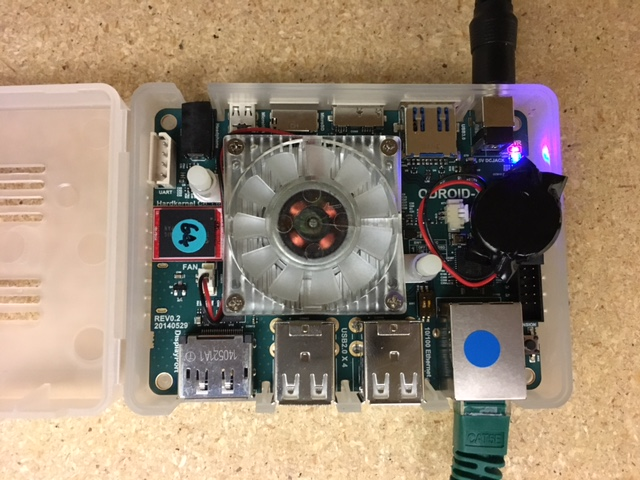
\includegraphics[width=.22\textwidth]{figures/odroid.png}
    \label{fig:odroid}
  }
  \subfloat[]
  {
    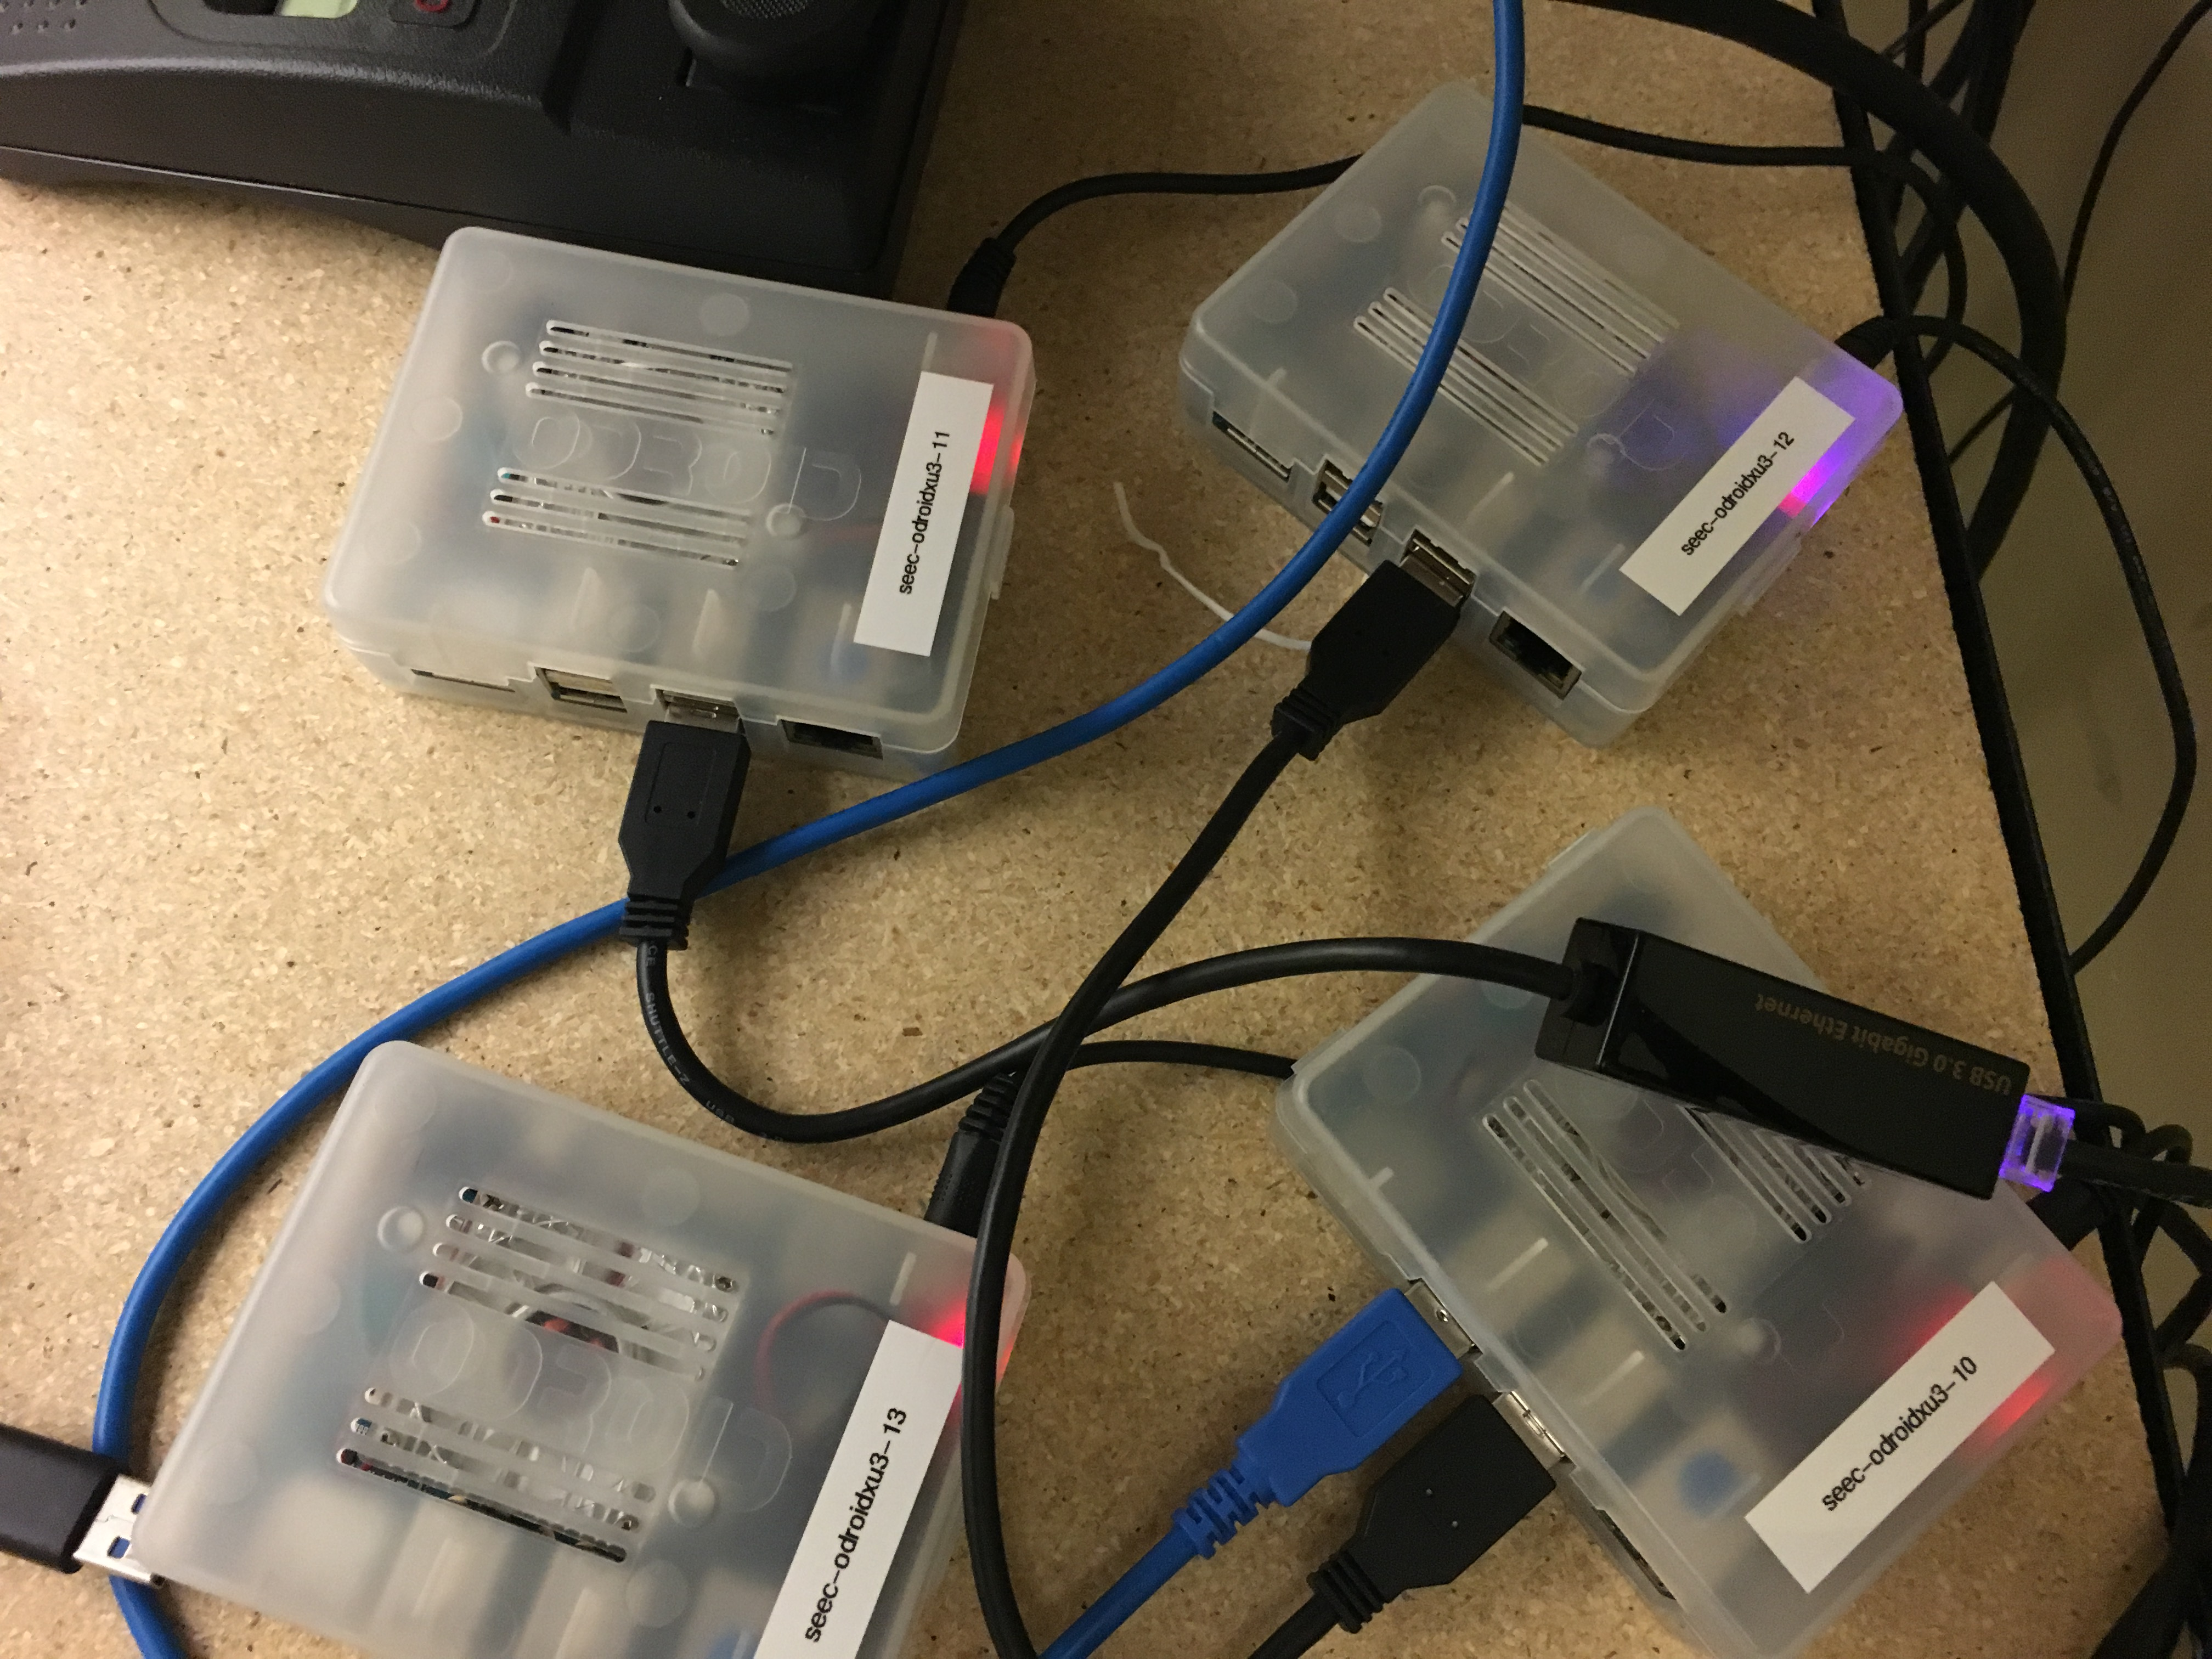
\includegraphics[width=.22\textwidth]{figures/odroidall.png}
    \label{fig:odroid_all}
  }
 \caption{ODROID-XU3 boards used in the evaluation.}
 \label{fig:odroidall}
\end{figure}

\subsection{Platform and Benchmarks}
We run streaming applications on four ODROID-XU3 devices running
Ubuntu 14.04, as shown in \figref{fig:odroidall}. The ODROIDs have
Samsung Exynos 5 Octa processors using the ARM big.LITTLE
architecture.  Each has 19 speed settings for the 4 big cores and 13
for 4 LITTLE cores.  Each board has an on-board power meter updated at
1/4 \ms intervals, this meter captures core, GPU, memory, and flash
drive power.  Each resource configuration (combination of big/LITTLE
cores and clock-speeds) has a different performance and power, which
is application-dependent.

We use 20 benchmarks from different suites including PARSEC
\cite{parsec}, Minebench \cite{minebench}, Rodinia \cite{rodinia}, and
STREAM \cite{stream}. \figref{fig:application_variety} shows the
variety of workloads indicated by the \emph{lack-of-fit} or the
absence of correlation between frequency and performance.
Applications with high lack-of-fit do not speed up with increasing
frequency---typical of memory bound applications. Applications with
low lack-of-fit do see increasing performance with increasing
clock-speed \cite{powerslope}.  Applications with intermediate
lack-of-fit tend to improve with increasing clock speed up to a point
and then see no further improvement.  Each application has an outer
loop which processes one unit in a data stream (\eg{} a point for
\texttt{kmeans} or a frame for \texttt{x264}). The application signals
the completion of processing a single stream element using a standard
API \cite{icac2010heartbeats}.  Performance targets are specified as
application-specific latencies for these stream elements.



\begin{figure}[t]
  \begin{tikzpicture}
\definecolor{s1}{RGB}{228, 26, 28}
\definecolor{s2}{RGB}{55, 126, 184}
\definecolor{s3}{RGB}{77, 175, 74}
\definecolor{s4}{RGB}{152, 78, 163}
\definecolor{s5}{RGB}{255, 127, 0}

\begin{groupplot}[
    group style={
        group name=plots,
        group size=1 by 1,
        xlabels at=edge top,
        xticklabels at=edge top,
        vertical sep=5pt
    },
axis x line* = top,
xlabel near ticks,
major x tick style = transparent,
height=3cm,
width=\columnwidth,
xmin=0,
xmax=9,
enlargelimits=false,
tick align = outside,
tick style={white},
ylabel style={align=center},
ytick=\empty,
xtick=\empty,
xticklabels={},
yticklabels={},
ymin=0,
ymax=1,
]
\nextgroupplot[ylabel={},
y label style={rotate=270},
ylabel shift={12mm},
]
\addplot[thick,solid, color=black] coordinates {(0,1) (22,1)};


\end{groupplot}

\begin{groupplot}[
    group style={
        group name=plots,
        group size=1 by 2,
        xlabels at=edge bottom,
        xticklabels at=edge bottom,
        vertical sep=5pt
    },
axis x line* = bottom,
xlabel near ticks,
major x tick style = transparent,
xlabel={},
height=3cm,
width=\columnwidth,
xmin=0,
xmax=21,
enlargelimits=false,
tick align = outside,
tick style={white},
ylabel style={align=center},
ytick=\empty,
ymin=0,
ymax=0.5,
ytick={0,0.1,0.3,0.5},
yticklabels={,0.1,0.3,0.5},
legend cell align=left, 
legend style={ column sep=1ex },
ymajorgrids,
grid style={dashed},
]


\nextgroupplot[ybar=\pgflinewidth,
bar width=2.0pt,
ylabel={\footnotesize \emph{lack-of-fit} \\ (1-adjustedR2)}, 
ylabel shift={0mm},
xticklabel shift={1pt},
x tick label style={rotate=35, anchor=east},
xtick={1,2,3,4,5,6,7,8,9,10,11,12,13,14,15,16,17,18,19,20,21},
xticklabels={
{\scriptsize $\mathsf{backprop}$},
{\scriptsize $\mathsf{bfs}$},
{\scriptsize $\mathsf{blackscholes}$},
{\scriptsize $\mathsf{bodytrack}$},
{\scriptsize $\mathsf{facesim}$},
{\scriptsize $\mathsf{ferret}$},
{\scriptsize $\mathsf{heartwall}$},
{\scriptsize $\mathsf{hotspot}$},
{\scriptsize $\mathsf{jacobi}$},
{\scriptsize $\mathsf{kmeans}$},
{\scriptsize $\mathsf{kmeansnf}$},
{\scriptsize $\mathsf{lavamd}$},
{\scriptsize $\mathsf{leukocyte}$},
{\scriptsize $\mathsf{lud}$},
{\scriptsize $\mathsf{nw}$},
{\scriptsize $\mathsf{sha}$},
{\scriptsize $\mathsf{srad}$},
{\scriptsize $\mathsf{stream_threads}$},
{\scriptsize $\mathsf{x264-ducks}$},
{\scriptsize $\mathsf{x264-native}$}},
]
\addplot[color=calnp,fill=calnp] table[x index=0,y index=1, col sep=space] {img/image_text/mem-compute.txt};

\end{groupplot}
\end{tikzpicture}
   \vskip -1em
   \caption{\emph{Lack-of-fit} for performance vs clock-speed. Lower
     lack-of-fit indicates a more compute-bound application, higher
     values indicate a memory-bound one.}
  \label{fig:application_variety}
\end{figure}


\subsection{Evaluation Metrics}
%\SYSTEM{} uses the model for power and performance and its controller
%actively uses this knowledge to meet the performance target. 
The latency targets represent performance requirements. To test a
variety of requirements, we run our applications with targets that
represent 50-90\% of the maximum speed and evaluate \SYSTEM{} under
each constraint. We quantify the performance reliability by measuring
the number of deadlines that were missed for each application and
performance target. If the application processes $n$ elements total
and $m$ of those elements took longer than the target latency we
compute deadline misses as:
\begin{equation}
deadline\, misses = 100\% \cdot \frac{m}{n}.
\end{equation}

We evaluate energy savings by constructing an oracle.  We run every
application in every resource configuration and record performance and
power for every stream element.  By post-processing this data we
determine the optimal resource configuration for each stream element
and performance target. To compare across applications, we normalize
energy:
\begin{equation}
  normalized\,energy = 100\% . \left( \frac{e_{measured}}{e_{optimal}} - 1 \right)
\end{equation}
where $e_{measured}$ is measured energy and $e_{optimal}$ is the
optimal energy produced by our oracle. We subtract 1, so that this
metric shows the percentage of energy over optimal.  

\subsection{Points of Comparison}
We compare \SYSTEM{} to a number of existing learning and control
approaches:
\begin{enumerate}
\item \textit{Race-to-idle}: This well known heuristic allocates all
  resources to the application to complete each stream element as fast
  as possible, then idles until the next element is available
  \cite{kim-cpsna,powerslope,heisner}.  This heuristic requires no
  knowledge of the application and never misses deadlines in a
  single-application scenario.
\item \textit{PID-Control}: This is a standard single-input
  (performance), multiple-output (big/LITTLE core counts and speeds)
  proportional-integral-controller representative of several that have
  been proposed for computer resource management
  \cite{Hellerstein2004a,METE}.  This controller is tuned to provide
  the best average case behavior across all applications and targets.
\item \textit{Online}: observes the new application in small number of
  configurations then performs polynomial multivariate regression to
  estimate unobserved configurations' behavior
  \cite{LEO,Li2006,Ponamarev}.
\item \textit{Offline}: does not observe any values for the current
  application---instead using previously observed applications to
  estimate power and performance as a linear regression
  \cite{PUPiL,LeeBrooks2006,CPR}.
\item \textit{Netflix}: is a matrix completion algorithm for the
  Netflix challenge. Variations of this approach allocate
  heterogeneous resources in data centers \cite{Paragon,quasar}.
\item \textit{HBM}: is a hierarchical Bayesian learner previously used
  to allocate resources to meet performance goals with minimal energy
  in server systems \cite{LEO}.
\item \textit{Adaptive-Control}: is a state-of-the-art, adaptive
  controller that meets application performance with minimal energy
  \cite{POET}.  This approach requires a user-specified model relating
  resource configuration to performance and power.  For this paper, we
  use the \emph{Offline} learner's predictions.  \PUNT{A recent study
    comparing ML and control techniques for resource allocation showed
    that there was no single best approach, but adaptive control had
    the best average behavior \cite{TAAS}.}
\end{enumerate}


\SYSTEM{} is a framework for combining different learners with the
\SYSTEM{} control system.  We compare the above baselines to four
different versions of \SYSTEM{}:
\begin{enumerate}
\item \textit{CALOREE-NoPole}: uses the HBM learner, but sets the pole
  to 0.  This baseline shows the importance of incorporating the
  confidence interval and learned variance into control. All other
  versions of \SYSTEM{} set the pole according to \secref{guarantees}.
\item \textit{CALOREE-online}: uses the online learner.
\item \textit{CALOREE-nuclear}: uses the Nuclear learner.
\item \textit{CALOREE-HBM}: uses the HBM learner.
\end{enumerate}

In all cases that require prior knowledge, we ensure that knowledge of
the application under test is never included in that set of prior
knowledge.  Specifically, we use leave-one-out cross validation: to
test application $x$, we form a set of all other applications, train
the learners, and then test on $x$.

\section{Experimental Evaluation}

\subsection{Performance and Energy for Single App}
%Setup

\begin{figure}[!th]
\centering
  \begin{tikzpicture}
\begin{centering}
\pgfplotstableread[col sep=space]{img/single-eff-summary.txt}{\datatableeff}
\pgfplotstableread[col sep=space]{img/single-lat-summary.txt}{\datatablelat}
\begin{groupplot}[
% MAKE SURE NO SPACE AROUND EQUALITY
    scatter/classes={
            OPTIMAL={mark=otimes*,OPTIMAL},
            RACE={mark=otimes*,RACE},
            CONTROL={mark=otimes*,CONTROL},
            ONLINE={mark=otimes*,ONLINE},
            OFFLINE={mark=otimes*,OFFLINE},
            NUCLEAR={mark=otimes*,NUCLEAR},
            HBM={mark=otimes*,HBM},
            ADAPT-CONTROL={mark=otimes*,ADAPT-CONTROL},
            CALOREE-NP={mark=otimes*,CALOREE-NP},
            ONLINE-ADAPT={mark=otimes*,ONLINE-ADAPT},
            NUCLEAR-ADAPT={mark=otimes*,NUCLEAR-ADAPT},
            HBM-ADAPT={mark=otimes*,HBM-ADAPT}},
    group style={
        group name=plots,
        group size=1 by 2,
        xlabels at=edge bottom,
        xticklabels at=edge bottom,
        vertical sep=5pt},
    enlargelimits=false,
    tick align = outside,
    tick style={white},
    ylabel style={align=center},
    unbounded coords=jump,
    grid=both,
]

\nextgroupplot[
        scale only axis,
        height=2cm,
        width=0.80\columnwidth,
        xlabel near ticks,
        xlabel = {},
        xmin = 0,
        xmax = 13,
        xtick={1,2,3,4,5,6,7,8,9,10,11,12,13},
        x tick label style={rotate=45, anchor = east, font=\tiny},
        ylabel={\tiny Deadline Misses (\%) \\ {\tiny (lower is better)}},    
        ytick pos=left
        ]
        \addplot[scatter, only marks ,thick, scatter src=explicit symbolic] table[x index=0,y index=3, meta=Benchmark] {\datatablelat};
        %\addplot[only marks, mark=diamond*, scatter src=explicit symbolic,  error bars/.cd, y dir=minus,  y explicit ] table [x index=0, y index=3, y error index=2, meta=Benchmark]  {\datatable};
        \addplot[only marks,mark=o,  scatter src=explicit symbolic,  error bars/.cd, y dir=plus,   y explicit] table [x index=0, y index=3, y error index=4, meta=Benchmark]  {\datatablelat};
        \addplot[only marks, mark=o, scatter src=explicit symbolic,  error bars/.cd, y dir=minus,  y explicit ] table [x index=0, y index=3, y error index=2, meta=Benchmark]  {\datatablelat};

\nextgroupplot[
        scale only axis,
        %grid=both,
        height=2cm,
        width=0.80\columnwidth,
        xlabel near ticks,
        xlabel = {},
        xmin = 0,
        xmax = 13,
        ylabel={\tiny Energy Over Optimal (\%) \\ {\tiny (lower is better)}},
        xticklabel shift={0pt},
        xtick={1,2,3,4,5,6,7,8,9,10,11,12,13},
        x tick label style={rotate=45, anchor = east, font=\tiny},
        %xticklabels from table={\datatableeff}{Benchmark},
        xticklabels={{\scriptsize $\mathsf{Optimal}$},
{\scriptsize $\mathsf{Race-to-idle}$},
{\scriptsize $\mathsf{PID-Control}$},
{\scriptsize $\mathsf{Online}$},
{\scriptsize $\mathsf{Offline}$},
{\scriptsize $\mathsf{Netflix}$},
{\scriptsize $\mathsf{HBM}$},
{\scriptsize $\mathsf{Adaptive-Control}$},
{\scriptsize $\mathsf{CALOREE-NoPole}$},
{\scriptsize $\mathsf{CALOREE-Online}$},
{\scriptsize $\mathsf{CALOREE-Netflix}$},
{\scriptsize $\mathsf{CALOREE-HBM}$}
},
]

        ]
        \addplot[scatter, only marks ,thick, scatter src=explicit symbolic] table[x index=0,y index=3, meta=Benchmark] {\datatableeff};
        \addplot[only marks,mark=o,  scatter src=explicit symbolic,  error bars/.cd, y dir=plus,   y explicit] table [x index=0, y index=3, y error index=2]  {\datatableeff};
        \addplot[only marks, mark=o, scatter src=explicit symbolic,  error bars/.cd, y dir=minus,  y explicit] table [x index=0, y index=3, y error index=4]  {\datatableeff};

\end{groupplot}
\end{centering}
\end{tikzpicture}

   \vskip -.5em
  \caption{Summary data for single-app scenario.}
  \label{fig:single-sum}
\end{figure}

We set a range of performance targets from 50-90\% of the maximum
achievable performance and measure the deadline misses and
energy over optimal for all points of comparison.
\figref{fig:single-sum} represents the summary results as an average
error across all targets for the single application scenario. This figure
shows two charts with the percentage of deadline misses in the top
chart and the energy over optimal in the bottom.  The dots show the
average for each technique, while the error bars show the minimum and
maximum values.  

Not surprisingly, race-to-idle meets all deadlines, but its
conservative resource allocation has the highest average energy
consumption. Among the prior learning approaches Nuclear has the
lowest average deadline misses (11\%), but with high energy (40\% more
than optimal), while the HBM has higher deadline misses (17\%) but
with significantly lower energy consumption (16\%). Adaptive control
achieves similar deadline misses (14\%) with lower average energy than
any of the prior learning approaches (12\%). \SYSTEM{} with no pole
misses 45\% of all deadlines, which is clearly unacceptable.


\begin{figure*}[t]
 \captionsetup[subfigure]{labelformat=empty}
  \subfloat[]
  {
    \begin{tikzpicture}
%\pgfplotstableread[col sep=space]{img/image_text/dyn-mape-0.5-v2.txt}{\datatablefive}
\pgfplotstableread[col sep=space]{img/image_text/dyn-lat-0.60-v3.txt}{\datatablesixty}
\pgfplotstableread[col sep=space]{img/image_text/dyn-lat-0.75-v3.txt}{\datatableseventyfive}
\pgfplotstableread[col sep=space]{img/image_text/dyn-lat-0.90-v3.txt}{\datatableninty}
\begin{groupplot}[
    group style={
        group name=plots,
        group size=1 by 3,
        xlabels at=edge bottom,
        xticklabels at=edge bottom,
        vertical sep=5pt
    },
axis x line* = bottom,
xlabel near ticks,
major x tick style = transparent,
xlabel={},
height=2.8cm,
width=0.88\textwidth,
xmin=0,
xmax=23,
enlargelimits=false,
tick align = outside,
tick style={white},
ylabel style={align=center},
ytick=\empty,
ymin=0,
ymax=30,
ytick={0,5,10,15,20},
yticklabels={,5,10,15,20},
legend cell align=left, 
legend style={ column sep=1ex },
ymajorgrids,
grid style={dashed},
]


\nextgroupplot[ybar=\pgflinewidth,
ylabel shift={0mm},
bar width=2.0pt,
legend entries = {{$\mathsf{Race-to-idle}$},
{$\mathsf{Netflix}$},
{$\mathsf{HBM}$},
{$\mathsf{POET}$},
{$\mathsf{CALOREE-HBM}$}},
legend style={draw=none, legend columns=6,at={(.5,1.7)},anchor=north},
ymin=0,
ymax=20,
ytick={0.0,5.0,10.0,15.0,20.0},
yticklabels={,5.0,10.0,15.0},
]

\addplot[color=RACE, fill=RACE]       table[x index=0,y index=3] {\datatablesixty};
\addplot[color=NETFLIX, fill=NETFLIX]     table[x index=0,y index=6] {\datatablesixty};
\addplot[color=HBM, fill=HBM]   table[x index=0,y index=7] {\datatablesixty};
\addplot[color=POET, fill=POET] table[x index=0,y index=9] {\datatablesixty};
\addplot[color=CALOREE-HBM, fill=CALOREE-HBM]     table[x index=0,y index=13] {\datatablesixty};
                                

\nextgroupplot[ybar=\pgflinewidth,
ylabel={\footnotesize MAPE  {\scriptsize (lower is better)}},
ylabel shift={0mm},
bar width=2.0pt,
ymin=0,
ymax=30,
ytick={0.0,10.0,20.0,30.0},
yticklabels={,10.0,20.0,30.0},
]

%\addplot[color=RACE,fill=RACE] table[x index=0,y index=4] {\datatableseventyfive};
%\addplot[color=HBM,fill=HBM]       table[x index=0,y index=7] {\datatableseventyfive};
%\addplot[color=ADAPT-CONTROL,fill=ADAPT-CONTROL] table[x index=0,y index=9] {\datatableseventyfive};
%\addplot[color=CALOREE-NP,fill=CALOREE-NP]   table[x index=0,y index=10] {\datatableseventyfive};
%\addplot[color=HBM-ADAPT,fill=HBM-ADAPT]       table[x index=0,y index=13] {\datatableseventyfive};
\addplot[color=RACE, fill=RACE]       table[x index=0,y index=3] {\datatableseventyfive};
\addplot[color=NETFLIX, fill=NETFLIX]     table[x index=0,y index=6] {\datatableseventyfive};
\addplot[color=HBM, fill=HBM]   table[x index=0,y index=7] {\datatableseventyfive};
\addplot[color=POET, fill=POET] table[x index=0,y index=9] {\datatableseventyfive};
\addplot[color=CALOREE-HBM, fill=CALOREE-HBM]     table[x index=0,y index=13] {\datatableseventyfive};

\nextgroupplot[ybar=\pgflinewidth,
bar width=2.0pt,
ylabel shift={0mm},
xticklabel shift={0pt},
ymin=0,
ymax=30,
ytick={0.0,10.0,20.0,30.0},
yticklabels={,10.0,20.0,30.0},
x tick label style={rotate=35, anchor=east},
xtick={1,2,3,4,5,6,7,8,9,10,11,12,13,14,15,16,17,18,19,20,21,22},
xticklabels={
{\scriptsize $\mathsf{backprop}$},
{\scriptsize $\mathsf{bfs}$},
{\scriptsize $\mathsf{blackscholes}$},
{\scriptsize $\mathsf{bodytrack}$},
{\scriptsize $\mathsf{facesim}$},
{\scriptsize $\mathsf{ferret}$},
{\scriptsize $\mathsf{heartwall}$},
{\scriptsize $\mathsf{hotspot}$},
{\scriptsize $\mathsf{jacobi}$},
{\scriptsize $\mathsf{kmeans}$},
{\scriptsize $\mathsf{kmeansnf}$},
{\scriptsize $\mathsf{lavamd}$},
{\scriptsize $\mathsf{leukocyte}$},
{\scriptsize $\mathsf{lud}$},
{\scriptsize $\mathsf{nw}$},
{\scriptsize $\mathsf{sha}$},
{\scriptsize $\mathsf{srad}$},
{\scriptsize $\mathsf{stream}$},
{\scriptsize $\mathsf{stream_threads}$},
{\scriptsize $\mathsf{x264-ducks}$},
{\scriptsize $\mathsf{x264-native}$},
{\scriptsize $\mathsf{Average}$}},
]

\addplot[color=RACE, fill=RACE]       table[x index=0,y index=3] {\datatableninty};
\addplot[color=NETFLIX, fill=NETFLIX]     table[x index=0,y index=6] {\datatableninty};
\addplot[color=HBM, fill=HBM]   table[x index=0,y index=7] {\datatableninty};
\addplot[color=POET, fill=POET] table[x index=0,y index=9] {\datatableninty};
\addplot[color=CALOREE-HBM, fill=CALOREE-HBM]     table[x index=0,y index=13] {\datatableninty};

\end{groupplot}
\begin{groupplot}[
    group style={
        group name=plots,
        group size=1 by 6,
        xlabels at=edge top,
        xticklabels at=edge top,
        vertical sep=5pt
    },
axis x line* = top,
xlabel near ticks,
major x tick style = transparent,
height=2.8cm,
width=0.88\textwidth,
xmin=0,
xmax=9,
enlargelimits=false,
tick align = outside,
tick style={white},
ylabel style={align=center},
ytick=\empty,
xtick=\empty,
xticklabels={},
yticklabels={},
ymin=0,
ymax=1,
]

\nextgroupplot[
ylabel shift={12mm},
ylabel style={rotate=270},
ylabel={$\mathsf{60\%}$},
]
\addplot[thick,solid, color=black] coordinates {(0,1) (22,1)};


\nextgroupplot[
ylabel shift={12mm},
ylabel={$\mathsf{75\%}$},
ylabel style={rotate=270},
]
\addplot[thick,solid, color=black] coordinates {(0,1) (22,1)};


\nextgroupplot[
ylabel shift={12mm},
ylabel={$\mathsf{90\%}$},
y label style={rotate=270},
]
\addplot[thick,solid, color=black] coordinates {(0,1) (22,1)};

\end{groupplot}

\end{tikzpicture}
  }
  \\
  \vskip -2.5em
  \subfloat[]
  {
    
\begin{tikzpicture}

\pgfplotstableread[col sep=tab]{img/image_text/wcet-eff-1.0.txt}{\datatableninty}
\begin{groupplot}[
    group style={
        group name=plots,
        group size=1 by 1,
        xlabels at=edge bottom,
        xticklabels at=edge bottom,
        vertical sep=5pt
    },
axis x line* = bottom,
xlabel near ticks,
major x tick style = transparent,
xlabel={},
height=3.0cm,
width=0.95\textwidth,
xmin=0,
xmax=15,
enlargelimits=false,
tick align = outside,
tick style={white},
ylabel style={align=center},
ytick=\empty,
ymin=0,
ymax=15,
ytick={0,5,10,15,20},
yticklabels={,5,10,15,20},
ylabel={\tiny Energy Above \\ {\tiny Optimal (\%)} \\ {\tiny (lower is better)}},
legend cell align=left, 
legend style={ column sep=1ex },
ymajorgrids,
grid style={dashed},
]

\nextgroupplot[ybar=\pgflinewidth,
bar width=4.0pt,
ylabel shift={0mm},
xticklabel shift={0pt},
ymin=0,
ymax=90,
ytick={0.0,30.0,60.0,90.0},
yticklabels={,30.0,60.0,90.0},
x tick label style={rotate=35, anchor=east},
xtick={1,2,3,4,5,6,7,8,9,10,11,12,13,14},
xticklabels={
{\tiny $\mathsf{bodytrack}$},
{\tiny $\mathsf{facesim}$},
{\tiny $\mathsf{ferret}$},
{\tiny $\mathsf{heartwall}$},
{\tiny $\mathsf{kmeans}$},
{\tiny $\mathsf{leukocyte}$},
{\tiny $\mathsf{lud}$},
{\tiny $\mathsf{radar}$},
{\tiny $\mathsf{sha}$},
{\tiny $\mathsf{srad}$},
{\tiny $\mathsf{stream}$},
{\tiny $\mathsf{x264-ducks}$},
{\tiny $\mathsf{x264-native}$},
{\tiny $\mathsf{Average}$}},
]

\addplot[color=black, fill=RACE]       table[x index=0,y index=3] {\datatableninty};
\addplot[color=black, fill=NETFLIX]     table[x index=0,y index=6] {\datatableninty};
\addplot[color=black, fill=HBM]   table[x index=0,y index=7] {\datatableninty};
\addplot[color=black, fill=POET] table[x index=0,y index=9] {\datatableninty};
\addplot[color=black, fill=CALOREE-HBM]     table[x index=0,y index=13] {\datatableninty};

\end{groupplot}


\end{tikzpicture}

  }
  \vskip -1em
  \label{fig:multi}
  \caption{Comparison of application performance error and energy for single application scenario.}
 \label{fig:odroidall}
\end{figure*}

When we allow \SYSTEM{} to adaptively tune its pole, however, we see
greatly improved results.  The best combination is \SYSTEM{} with the
HBM, which misses only 5.5\% of deadlines on average, while consuming
just 4.4\% more energy than optimal.  These numbers represent large
improvements in both performance reliability and energy efficiency
compared to prior approaches.  The other learners paired with
\SYSTEM{} achieve similar results to the prior adaptive control
approach.

The summary data shows us that the best prior approaches are
race-to-idle, HBM, and adaptive control.
\figsref{fig:single-perf}{fig:single-energy} show the detailed results
for the 60, 75, and 90\% targets comparing the best of these prior
approaches to \SYSTEM{} with no pole and \SYSTEM{} coupled with the
HBM---other data has been omitted for space.  The benchmarks are
shown on the x-axis; the y-axis shows the number of deadline misses
and the normalized energy, respectively.

%In addition to providing better average case behavior, \SYSTEM{}
%provides significantly better worst case behavior.  


\subsection{Performance and Energy for Multiple Apps}
\begin{figure}[!t]
\centering
  \begin{tikzpicture}
\begin{centering}
\pgfplotstableread[col sep=space]{img/ma-eff-summary.txt}{\datatableeff}
\pgfplotstableread[col sep=space]{img/ma-lat-summary.txt}{\datatablelat}
\begin{groupplot}[
% MAKE SURE NO SPACE AROUND EQUALITY
    scatter/classes={
            OPTIMAL={mark=otimes*,OPTIMAL},
            RACE={mark=otimes*,RACE},
            CONTROL={mark=otimes*,CONTROL},
            ONLINE={mark=otimes*,ONLINE},
            OFFLINE={mark=otimes*,OFFLINE},
            NUCLEAR={mark=otimes*,NUCLEAR},
            HBM={mark=otimes*,HBM},
            ADAPT-CONTROL={mark=otimes*,ADAPT-CONTROL},
            CALOREE-NP={mark=otimes*,CALOREE-NP},
            ONLINE-ADAPT={mark=otimes*,ONLINE-ADAPT},
            NUCLEAR-ADAPT={mark=otimes*,NUCLEAR-ADAPT},
            HBM-ADAPT={mark=otimes*,HBM-ADAPT}},
    group style={
        group name=plots,
        group size=1 by 2,
        xlabels at=edge bottom,
        xticklabels at=edge bottom,
        vertical sep=5pt},
    enlargelimits=false,
    tick align = outside,
    tick style={white},
    ylabel style={align=center},
    unbounded coords=jump,
    grid=both,
]

\nextgroupplot[
        scale only axis,
        height=2cm,
        width=0.80\columnwidth,
        xlabel near ticks,
        xlabel = {},
        xmin = 0,
        xmax = 13,
        xtick={1,2,3,4,5,6,7,8,9,10,11,12,13},
        x tick label style={rotate=45, anchor = east, font=\tiny},
        ylabel={\footnotesize \% Latency \\ {\scriptsize (lower is better)}},    
        ytick pos=left
        ]
        \addplot[scatter, only marks ,thick, scatter src=explicit symbolic] table[x index=0,y index=3, meta=Benchmark] {\datatablelat};
        %\addplot[only marks, mark=diamond*, scatter src=explicit symbolic,  error bars/.cd, y dir=minus,  y explicit ] table [x index=0, y index=3, y error index=2, meta=Benchmark]  {\datatable};
        \addplot[only marks,mark=o,  scatter src=explicit symbolic,  error bars/.cd, y dir=plus,   y explicit] table [x index=0, y index=3, y error index=4, meta=Benchmark]  {\datatablelat};
        \addplot[only marks, mark=o, scatter src=explicit symbolic,  error bars/.cd, y dir=minus,  y explicit ] table [x index=0, y index=3, y error index=2, meta=Benchmark]  {\datatablelat};

\nextgroupplot[
        scale only axis,
        %grid=both,
        height=2cm,
        width=0.80\columnwidth,
        xlabel near ticks,
        xlabel = {},
        xmin = 0,
        xmax = 13,
        ylabel={\footnotesize \% Energy efficiency\\ {\scriptsize (lower is better)}},
        xticklabel shift={0pt},
        xtick={1,2,3,4,5,6,7,8,9,10,11,12,13},
        x tick label style={rotate=45, anchor = east, font=\tiny},
        %xticklabels from table={\datatableeff}{Benchmark},
        xticklabels={{\scriptsize $\mathsf{Optimal}$},
{\scriptsize $\mathsf{Race-to-idle}$},
{\scriptsize $\mathsf{PID-Control}$},
{\scriptsize $\mathsf{Online}$},
{\scriptsize $\mathsf{Offline}$},
{\scriptsize $\mathsf{Netflix}$},
{\scriptsize $\mathsf{HBM}$},
{\scriptsize $\mathsf{POET}$},
{\scriptsize $\mathsf{CALOREE-NoPole}$},
{\scriptsize $\mathsf{CALOREE-Online}$},
{\scriptsize $\mathsf{CALOREE-Netflix}$},
{\scriptsize $\mathsf{CALOREE-HBM}$}
}       
]
        \addplot[scatter, only marks ,thick, scatter src=explicit symbolic] table[x index=0,y index=3, meta=Benchmark] {\datatableeff};
        \addplot[only marks,mark=o,  scatter src=explicit symbolic,  error bars/.cd, y dir=plus,   y explicit] table [x index=0, y index=3, y error index=2]  {\datatableeff};
        \addplot[only marks, mark=o, scatter src=explicit symbolic,  error bars/.cd, y dir=minus,  y explicit] table [x index=0, y index=3, y error index=4]  {\datatableeff};

\end{groupplot}
\end{centering}
\end{tikzpicture}

   \vskip -.5em
  \caption{Summary data for multi-app scenario.}
  \label{fig:multi-sum}
\end{figure}

We again launch each benchmark with a performance target (using the
same targets as the prior study).  Halfway through execution, we start
another application randomly drawn from our benchmark set, which we
bind to one big core, which interferes with the application \SYSTEM{}
is controlling.  Delivering performance to the original application in
this dynamic scenario tests \SYSTEM{}'s ability to react to
environmental changes.

\begin{figure*}[t]
 \captionsetup[subfigure]{labelformat=empty}
  \subfloat[]
  {
    \begin{tikzpicture}


\begin{groupplot}[
    group style={
        group name=plots,
        group size=1 by 3,
        xlabels at=edge bottom,
        xticklabels at=edge bottom,
        vertical sep=5pt
    },
axis x line* = bottom,
xlabel near ticks,
major x tick style = transparent,
xlabel={},
height=2.8cm,
width=0.88\textwidth,
xmin=0,
xmax=23,
enlargelimits=false,
tick align = outside,
tick style={white},
ylabel style={align=center},
ytick=\empty,
ymin=0,
ymax=30,
ytick={0,5,10,15,20},
yticklabels={,5,10,15,20},
legend cell align=left, 
legend style={ column sep=1ex },
ymajorgrids,
grid style={dashed},
]



\nextgroupplot[ybar=\pgflinewidth,
ylabel shift={0mm},
bar width=2.0pt,
legend entries = {{$\mathsf{Online}$},{$\mathsf{Offline}$},{$\mathsf{LEO}$},{$\mathsf{POET}$},{$\mathsf{\SYSTEM{}-NP}$},{$\mathsf{\SYSTEM{}}$}},
legend style={draw=none,legend columns=6,at={(.5,1.7)},anchor=north},
ymin=0,
ymax=20,
ytick={0.0,5.0,10.0,15.0,20.0},
yticklabels={,5.0,10.0,15.0},
]

\addplot[color=on,fill=on]  table[x index=0,y index=3, col sep=space] {img/image_text/ma-err-0.5-v2.txt};
\addplot[color=off,fill=off]  table[x index=0,y index=4, col sep=space] {img/image_text/ma-err-0.5-v2.txt};
\addplot[color=leo,fill=leo]  table[x index=0,y index=5, col sep=space] {img/image_text/ma-err-0.5-v2.txt};
\addplot[color=poet,fill=poet]  table[x index=0,y index=6, col sep=space] {img/image_text/ma-err-0.5-v2.txt};
\addplot[color=calnp,fill=calnp]  table[x index=0,y index=7, col sep=space] {img/image_text/ma-err-0.5-v2.txt};
\addplot[color=cal,fill=cal]  table[x index=0,y index=8, col sep=space] {img/image_text/ma-err-0.5-v2.txt};

\nextgroupplot[ybar=\pgflinewidth,
ylabel={\footnotesize MAPE  {\scriptsize (lower is better)}},
ylabel shift={0mm},
bar width=2.0pt,
ymin=0,
ymax=30,
ytick={0.0,10.0,20.0,30.0},
yticklabels={,10.0,20.0,30.0},
]

\addplot[color=on,fill=on]  table[x index=0,y index=3, col sep=space] {img/image_text/ma-err-0.7-v2.txt};
\addplot[color=off,fill=off]  table[x index=0,y index=4, col sep=space] {img/image_text/ma-err-0.7-v2.txt};
\addplot[color=leo,fill=leo]  table[x index=0,y index=5, col sep=space] {img/image_text/ma-err-0.7-v2.txt};
\addplot[color=poet,fill=poet]  table[x index=0,y index=6, col sep=space] {img/image_text/ma-err-0.7-v2.txt};
\addplot[color=calnp,fill=calnp]  table[x index=0,y index=7, col sep=space] {img/image_text/ma-err-0.7-v2.txt};
\addplot[color=cal,fill=cal]  table[x index=0,y index=8, col sep=space] {img/image_text/ma-err-0.7-v2.txt};

\nextgroupplot[ybar=\pgflinewidth,
bar width=2.0pt,
ylabel shift={0mm},
xticklabel shift={0pt},
ymin=0,
ymax=30,
ytick={0.0,10.0,20.0,30.0},
yticklabels={,10.0,20.0,30.0},
x tick label style={rotate=35, anchor=east},
xtick={1,2,3,4,5,6,7,8,9,10,11,12,13,14,15,16,17,18,19,20,21,22},
xticklabels={
{\scriptsize $\mathsf{backprop}$},
{\scriptsize $\mathsf{bfs}$},
{\scriptsize $\mathsf{blackscholes}$},
{\scriptsize $\mathsf{bodytrack}$},
{\scriptsize $\mathsf{facesim}$},
{\scriptsize $\mathsf{ferret}$},
{\scriptsize $\mathsf{heartwall}$},
{\scriptsize $\mathsf{hotspot}$},
{\scriptsize $\mathsf{jacobi}$},
{\scriptsize $\mathsf{kmeans}$},
{\scriptsize $\mathsf{kmeansnf}$},
{\scriptsize $\mathsf{lavamd}$},
{\scriptsize $\mathsf{leukocyte}$},
{\scriptsize $\mathsf{lud}$},
{\scriptsize $\mathsf{nw}$},
{\scriptsize $\mathsf{sha}$},
{\scriptsize $\mathsf{srad}$},
{\scriptsize $\mathsf{stream}$},
{\scriptsize $\mathsf{stream_threads}$},
{\scriptsize $\mathsf{x264-ducks}$},
{\scriptsize $\mathsf{x264-native}$},
{\scriptsize $\mathsf{\mathbf{Average}}$}},
]

\addplot[color=on,fill=on]  table[x index=0,y index=3, col sep=space] {img/image_text/ma-err-0.9-v2.txt};
\addplot[color=off,fill=off]  table[x index=0,y index=4, col sep=space] {img/image_text/ma-err-0.9-v2.txt};
\addplot[color=leo,fill=leo]  table[x index=0,y index=5, col sep=space] {img/image_text/ma-err-0.9-v2.txt};
\addplot[color=poet,fill=poet]  table[x index=0,y index=6, col sep=space] {img/image_text/ma-err-0.9-v2.txt};
\addplot[color=calnp,fill=calnp]  table[x index=0,y index=7, col sep=space] {img/image_text/ma-err-0.9-v2.txt};
\addplot[color=cal,fill=cal]  table[x index=0,y index=8, col sep=space] {img/image_text/ma-err-0.9-v2.txt};

\end{groupplot}
\begin{groupplot}[
    group style={
        group name=plots,
        group size=1 by 6,
        xlabels at=edge top,
        xticklabels at=edge top,
        vertical sep=5pt
    },
axis x line* = top,
xlabel near ticks,
major x tick style = transparent,
height=2.8cm,
width=0.88\textwidth,
xmin=0,
xmax=9,
enlargelimits=false,
tick align = outside,
tick style={white},
ylabel style={align=center},
ytick=\empty,
xtick=\empty,
xticklabels={},
yticklabels={},
ymin=0,
ymax=1,
]

\nextgroupplot[
ylabel shift={12mm},
ylabel style={rotate=270},
ylabel={$\mathsf{50\%}$},
]
\addplot[thick,solid, color=black] coordinates {(0,1) (22,1)};

\nextgroupplot[
ylabel shift={12mm},
ylabel={$\mathsf{70\%}$},
y label style={rotate=270},
]
\addplot[thick,solid, color=black] coordinates {(0,1) (22,1)};

\nextgroupplot[
ylabel shift={12mm},
ylabel={$\mathsf{90\%}$},
y label style={rotate=270},
]
\addplot[thick,solid, color=black] coordinates {(0,1) (22,1)};

\end{groupplot}
\end{tikzpicture}
  }
  \\
  \vskip -2.5em
  \subfloat[]
  {
    \begin{tikzpicture}
%\pgfplotstableread[col sep=space]{img/image_text/ma-eff-0.60-v4.txt}{\datatablesixty}
%\pgfplotstableread[col sep=space]{img/image_text/ma-eff-0.75-v4.txt}{\datatableseventy}
\pgfplotstableread[col sep=space]{img/image_text/wcet-ma-eff-1.0.txt}{\datatableeighty}
\begin{groupplot}[
    group style={
        group name=plots,
        group size=1 by 1,
        xlabels at=edge bottom,
        xticklabels at=edge bottom,
        vertical sep=5pt
    },
axis x line* = bottom,
xlabel near ticks,
major x tick style = transparent,
xlabel={},
height=3.0cm,
width=0.95\textwidth,
xmin=0,
xmax=15,
enlargelimits=false,
tick align = outside,
tick style={white},
ylabel style={align=center},
ytick=\empty,
ymin=0,
ymax=30,
ytick={0,5,10,15,20},
yticklabels={,5,10,15,20},
legend cell align=left,
legend style={ column sep=1ex },
ymajorgrids,
grid style={dashed},
]

\nextgroupplot[ybar=\pgflinewidth,
bar width=3.0pt,
ylabel shift={0mm},
ylabel={\tiny Energy Above Optimal \\ {\tiny (lower is better)}},
xticklabel shift={0pt},
ymin=0,
ymax=90,
ytick={0.0,30.0,60.0,90.0},
yticklabels={,30.0,60.0,90.0},
x tick label style={rotate=35, anchor=east},
xtick={1,2,3,4,5,6,7,8,9,10,11,12,13,14,15,16,17,18,19,20,21,22},
xticklabels={
{\scriptsize $\mathsf{bodytrack}$},
{\scriptsize $\mathsf{facesim}$},
{\scriptsize $\mathsf{ferret}$},
{\scriptsize $\mathsf{heartwall}$},
{\scriptsize $\mathsf{kmeans}$},
{\scriptsize $\mathsf{leukocyte}$},
{\scriptsize $\mathsf{lud}$},
{\scriptsize $\mathsf{radar}$},
{\scriptsize $\mathsf{sha}$},
{\scriptsize $\mathsf{srad}$},
{\scriptsize $\mathsf{stream}$},
{\scriptsize $\mathsf{x264-ducks}$},
{\scriptsize $\mathsf{x264-native}$},
{\scriptsize $\mathsf{Average}$}},
]
\addplot[color=RACE, fill=RACE]       table[x index=0,y index=3] {\datatableeighty};
\addplot[color=NETFLIX, fill=NETFLIX]     table[x index=0,y index=6] {\datatableeighty};
\addplot[color=HBM, fill=HBM]   table[x index=0,y index=7] {\datatableeighty};
\addplot[color=POET, fill=POET] table[x index=0,y index=9] {\datatableeighty};
\addplot[color=CALOREE-HBM, fill=CALOREE-HBM]     table[x index=0,y index=13] {\datatableeighty};

\end{groupplot}

\end{tikzpicture}

  }
  \vskip -1em
  \label{fig:multi}
  \caption{Comparison of application performance error and energy for multiple application scenario.}
 \label{fig:odroidall}
\end{figure*}


\figref{fig:multi-sum} summarizes the results as the average number of
deadline misses and energy over optimal for all approaches.  We note
that some targets are unachievable for some applications. Due to these
unachievable targets, both optimal and race-to-idle show some deadline
misses. Race-to-idle misses more deadlines than optimal because it
cannot make use of LITTLE cores to do some work, it simply continues
using all big cores despite the degraded performance due to the second
application.  In fact, most approaches do badly in this
scenario---even adaptive control misses 50\% of the deadlines.
\SYSTEM{} with the HBM produces the lowest deadline misses with an
average of 20\%, which is only 5\% more than optimal.  It also
produces the second lowest energy, using slightly more than
race-to-idle because it uses LITTLE cores to make up for some work
that cannot be done on a big core due to the second application.
\figsref{fig:multi-perf}{fig:multi-energy} shows the detailed results.
The 90\% target is generally not reachable in this scenario as it
would require the controlled application to have exclusive use of all
big cores. \TODO{Hank: I am thinking that we subtract out the optimal
  number of deadline misses here.}



\PUNT{
\subsection{Multiapp Details for \texttt{bodytrack}}
To demonstrate \SYSTEM{} in this dynamic environment we look at the
specific example of \texttt{bodytrack} with a 70\% target, shown in
\figref{fig:bodytrack-multiapp} with time on the x-axis and
performance/power on the y-axis.  Performance is normalized to the
target.  There is a curve for each of HBM, Adaptive-Control, and
\SYSTEM{}-HBM. The vertical dashed line shows the point where the
second application starts.

\PUNT{This example illustrates \SYSTEM{}'s benefits over prior
  approaches that use only control or learning.  There are two key
  regions in the figures, the times before the second application
  starts (on the left of the vertical dashed line) and the times after
  (on the right).}  

Before the second application starts, both HBM and \SYSTEM{} track the
target and keeping energy low.  In contrast, Adaptive-Control produces
oscillating performance (and thus power) because its generic control
model does not capture \texttt{bodytrack}'s LITTLE core performance.
After the second application starts, Adaptive-Control and \SYSTEM{}
recognize the performance has changed and adjust resource usage.
\SYSTEM{} does a slightly better job tracking the change, producing
fewer oscillations.  HBM cannot adjust to the change as it computes
the optimal configuration once at the beginning of the application.
\SYSTEM{} with the HBM produces better results than the HBM alone
because it reacts to the change; it produces better results than
Adaptive-Control because it has captured the complex
application-specific behavior on this system.


\begin{figure}[t]
  \begin{tikzpicture}
\begin{centering}


\begin{groupplot}[
    group style={
        group name=plots,
        group size=1 by 2,
        xlabels at=edge bottom,
        xticklabels at=edge bottom,
        vertical sep=5pt
    },
height=3.5cm,
width=0.95\columnwidth,
xmajorgrids,
ymajorgrids,
grid style={dashed},
xmin=0,
xmax=260,
yticklabel pos=left,
enlargelimits=false,
tick align = outside,
tick style={white},
xticklabel shift={-5pt},
yticklabel shift={-5pt},
ylabel shift={-2pt},
ylabel style={align=center},
unbounded coords=jump,
]

\nextgroupplot[ylabel={\footnotesize Performance \\ (Normalized)}, % Performance
ytick={0.0,0.5,1.0,1.5,2.0},
yticklabels={,0.5,1.0,1.5,2.0},
yticklabel style={font=\footnotesize},
ymin=0,
ymax=1.5,
legend entries={{$\mathsf{POET}$},{$\mathsf{LEO}$},{{$\mathsf{\SYSTEM{}}$}}},
legend style={draw=none,at={(0.5,1.4)},anchor=north,legend columns=4,line width=5pt},
]

\addplot[thick, solid, color=poet, mark=none,each nth point=5] table[x index=0,y index=1,col sep=space] {img/bodytrack/poet2-BODYTRACK.txt};
\addplot[thick, solid, color=leo, mark=none,each nth point=5] table[x index=0,y index=1,col sep=space] {img/bodytrack/leo2-BODYTRACK.txt};
\addplot[thick, solid, color=cal, mark=none,each nth point=5] table[x index=0,y index=1,col sep=space] {img/bodytrack/leopoet2-BODYTRACK.txt};
\addplot[thick, dashed, black] coordinates {(130,0) (130, 2)};

\nextgroupplot[ylabel={\footnotesize Power \\ (Watts)}, % Power
ytick={2.0,4.0,6.0},
yticklabels={0.0,2.0,4.0,6.0},
yticklabel style={font=\footnotesize},
ymin=0,
ymax=6.0,
xlabel={\footnotesize $time$ [frame]},
xlabel near ticks,
]
\addplot[thick, solid, color=poet, mark=none,each nth point=5] table[x index=0,y index=2,col sep=space] {img/bodytrack/poet2-BODYTRACK.txt};
\addplot[thick, solid, color=leo, mark=none,each nth point=5] table[x index=0,y index=2,col sep=space] {img/bodytrack/leo2-BODYTRACK.txt};
\addplot[thick, solid, color=cal, mark=none,each nth point=5] table[x index=0,y index=2,col sep=space] {img/bodytrack/leopoet2-BODYTRACK.txt};
\addplot[thick, dashed, black] coordinates {(130,0) (130, 6)};
\end{groupplot}
\end{centering}

\end{tikzpicture}

   \vskip -.5em
  \caption{Time series of \texttt{Bodytrack} with phase change caused by multiple applications running.}
  \label{fig:bodytrack-multiapp}
\end{figure}
}

\subsection{Adapting to Phase Changes}
\begin{figure}[!h]
  \begin{tikzpicture}
\begin{centering}

\begin{groupplot}[
    group style={
        group name=plots,
        group size=1 by 2,
        xlabels at=edge bottom,
        xticklabels at=edge bottom,
        vertical sep=5pt
    },
height=3.cm,
width=0.95\columnwidth,
xmajorgrids,
ymajorgrids,
grid style={dashed},
xmin=0,
xmax=1000,
yticklabel pos=left,
enlargelimits=false,
tick align = outside,
tick style={white},
xticklabel shift={-5pt},
yticklabel shift={-5pt},
ylabel shift={-2pt},
ylabel style={align=center},
unbounded coords=jump,
]

\nextgroupplot[ylabel={\footnotesize Performance \\ (Normalized)}, % Performance
ytick={0.0,0.5,1.0,1.5,2.0},
yticklabels={,0.5,1.0,1.5,2.0},
yticklabel style={font=\footnotesize},
ymin=0,
ymax=1.5,
%legend entries={{$\mathsf{POET}$},{$\mathsf{HBM}$},{{$\mathsf{CALOREE-HBM}$}}},
legend entries={{$\mathsf{Adaptive-Control}$},{{$\mathsf{CALOREE-HBM}$}}},
legend style={draw=none,at={(0.5,1.5)},anchor=north,legend columns=4,line width=5pt},
]
\addplot[thick, solid, color=ADAPT-CONTROL, mark=none,each nth point=10] table[x index=0,y index=1,col sep=space] {img/x264-native-ducks/poet-x264.txt};
%\addplot[thick, solid, color=HBM, mark=none,each nth point=10] table[x index=0,y index=1,col sep=space] {img/x264-native-ducks/leo-x264.txt};
\addplot[thick, solid, color=HBM-ADAPT, mark=none,each nth point=10] table[x index=0,y index=1,col sep=space] {img/x264-native-ducks/leopoet-x264.txt};
\addplot[thick, dashed, black] coordinates {(500,0) (500, 2)};

\nextgroupplot[ylabel={\footnotesize Power \\ (Watts)}, % Power
ytick={0.0,1.0,2.0,3.0,4.0,5.0},
yticklabels={,1.0,2.0,3.0,4.0,5.0},
yticklabel style={font=\footnotesize},
ymin=0,
ymax=5,
xlabel={\footnotesize $time$ [frame]},
xlabel near ticks,
%xticklabels={,0,60,120,240,360,480},
]
\addplot[thick, solid, color=ADAPT-CONTROL, mark=none,each nth point=10] table[x index=0,y index=2,col sep=space] {img/x264-native-ducks/poet-x264.txt};
%\addplot[thick, solid, color=HBM, mark=none,each nth point=10] table[x index=0,y index=2,col sep=space] {img/x264-native-ducks/leo-x264.txt};
\addplot[thick, solid, color=HBM-ADAPT, mark=none,each nth point=10] table[x index=0,y index=2,col sep=space] {img/x264-native-ducks/leopoet-x264.txt};
\addplot[thick, dashed, black] coordinates {(500,0) (500, 5)};
\end{groupplot}
\end{centering}
\end{tikzpicture}

   \vskip -.5em
  \caption{Controlling \texttt{x264} through scene changes.}
  \label{fig:x264-phase-change}
\end{figure}
We compare \SYSTEM{} and Adaptive-Control reacting to input
variations.  \figref{fig:x264-phase-change} shows the \texttt{x264}
video encoder application with 2 different phases caused by a scene
change in the input that occurs at the $500^{th}$ frame. The first
scene is difficult and the second one is significantly easier.  In the
first scene, \SYSTEM{} is closer to the desired performance (1 in the
figure) and operates at a lower power state compared to
Adaptive-Control. Adaptive-Control is operating at a configuration not
on the Pareto frontier of power and performance.  When the input
changes, \SYSTEM{} is still meets the performance target with far less
fluctuations compared to Adaptive-Control.


\subsection{The Pole's Importance}
%\TODO{Add the LAVAMD contour plot?}  
\begin{figure}
\centering
  \subfloat[]
  {
    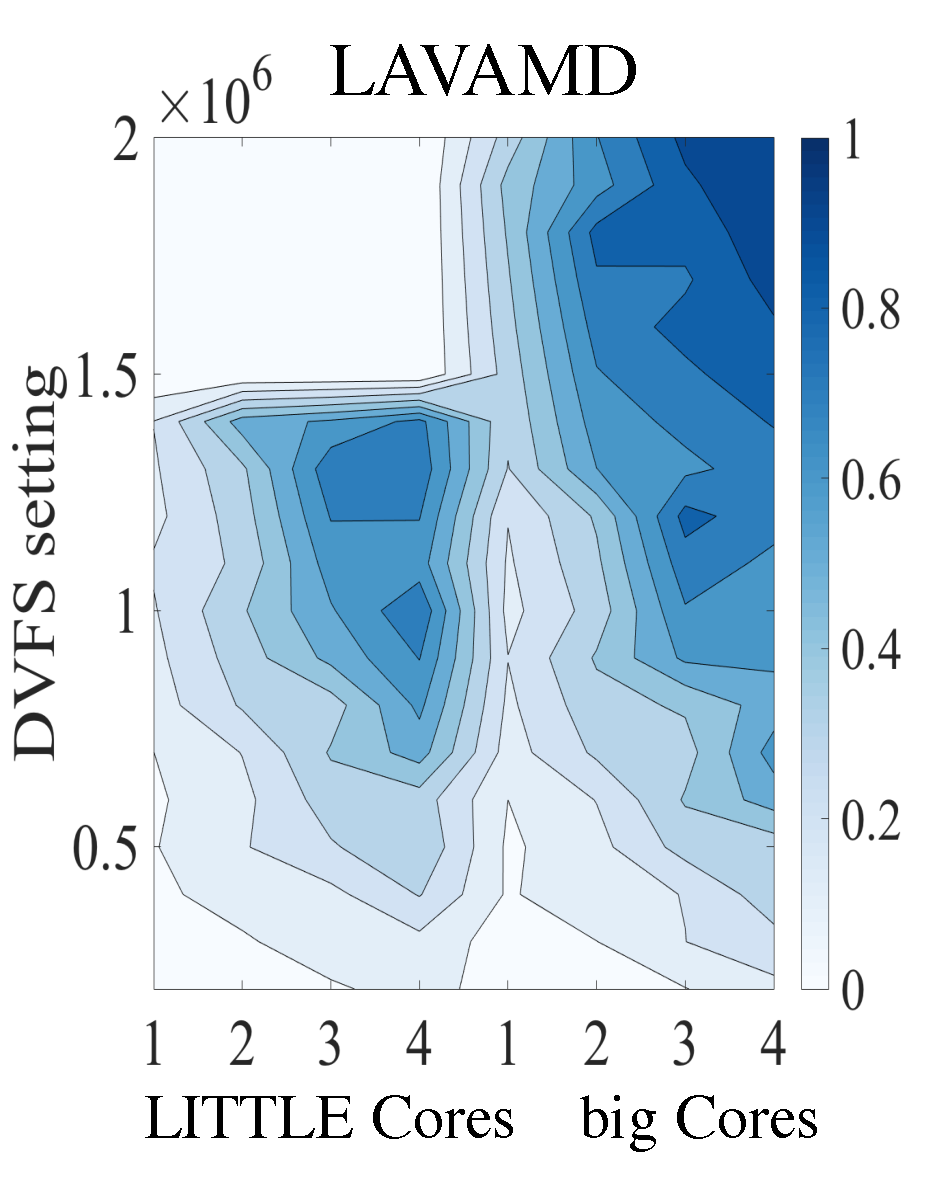
\includegraphics[width=.2\textwidth]{figures/lavamd2.pdf}
    \label{fig:lavamd}
  }
  \subfloat[]
  {
    \begin{tikzpicture}
\begin{centering}

\definecolor{s1}{RGB}{228, 26, 28}
\definecolor{s2}{RGB}{55, 126, 184}
\definecolor{s3}{RGB}{77, 175, 74}
\definecolor{s4}{RGB}{152, 78, 163}
\definecolor{s5}{RGB}{255, 127, 0}

\begin{groupplot}[
    group style={
        group name=plots,
        group size=1 by 2,
        xlabels at=edge bottom,
        xticklabels at=edge bottom,
        vertical sep=5pt
    },
height=3.5cm,
width=0.95\columnwidth,
xmajorgrids,
ymajorgrids,
grid style={dashed},
xmin=0,
xmax=500,
yticklabel pos=left,
enlargelimits=false,
tick align = outside,
tick style={white},
xticklabel shift={-5pt},
yticklabel shift={-5pt},
ylabel shift={-2pt},
ylabel style={align=center},
unbounded coords=jump,
]

\nextgroupplot[ylabel={\footnotesize Performance \\ (Normalized)}, % Performance
%xtick={0,500,1000,1500,2000,2500,3000,3500,4000,4500},
ytick={0.0,0.5,1.0,1.5,2.0},
yticklabels={,0.5,1.0,1.5,2.0},
%xtick={0,30,60,120,160,200,240,280,320,480},
%xticklabels={,0,30,60,120,160,200,240,280,320,480},
yticklabel style={font=\footnotesize},
ymin=0,
ymax=2.0,
legend entries={{$\mathsf{\SYSTEM{}-NP}$},{{$\mathsf{\SYSTEM{}}$}}},
legend style={draw=none,at={(0.5,1.4)},anchor=north,legend columns=4,line width=5pt},
]

\addplot[thick, solid, color=s5] table[x index=0,y index=1,col sep=space] {img/pole/leo-poet-np-LAVAMD.txt};
\addplot[thick, solid, color=s3] table[x index=0,y index=1,col sep=space] {img/pole/leo-poet-LAVAMD.txt};
%\addplot[thick, solid, color=s3] table[x index=0,y index=1,col sep=space] {img/x264-native-ducks/leopoet.txt};

%\addplot[thick, solid, color=s3] table[x index=0,y index=1,col sep=tab] {img/x264-phases-clover-dvfs.txt};
%\addplot[thick, solid, color=s4] table[x index=0,y index=1,col sep=tab] {img/x264-phases-clover-copper.txt};
%\addplot[thick, solid, black] coordinates {(0, 1) (4500, 1)};
\addplot[thick, dashed, black] coordinates {(250,0) (250, 2)};
%\addplot[thick, dashed, black] coordinates {(3000,0) (3000, 2)};


\nextgroupplot[ylabel={\footnotesize Power \\ (Watts)}, % Power
ytick={0.0,2.0,4.0,6.0},
yticklabels={,2.0,4.0,6.0},
yticklabel style={font=\footnotesize},
ymin=0,
ymax=6.0,
xlabel={\footnotesize $time$ [frame]},
xlabel near ticks,
%xtick={0,500,1000,1500,2000,2500,3000,3500,4000,4500},
%xtick={0,30,60,120,160,200,240,280,320,480},
xticklabels={,0,100,200,300,400,500},
%xticklabel style={font=\footnotesize},
]

\addplot[thick, solid, color=s5] table[x index=0,y index=2,col sep=space] {img/pole/leo-poet-np-LAVAMD.txt};
\addplot[thick, solid, color=s3] table[x index=0,y index=2,col sep=space] {img/pole/leo-poet-LAVAMD.txt};
%\addplot[thick, solid, color=s3] table[x index=0,y index=2,col sep=space] {img/x264-native-ducks/leopoet.txt};
%\addplot[thick, solid, color=s3] table[x index=0,y index=2,col sep=tab] {img/x264-phases-clover-dvfs.txt};
%\addplot[thick, solid, color=s4] table[x index=0,y index=2,col sep=tab] {img/x264-phases-clover-copper.txt};
%\addplot[thick, dashed, black] coordinates {(1500,0) (1500, 250)};
%\addplot[thick, dashed, black] coordinates {(3000,0) (3000, 250)};
\addplot[thick, dashed, black] coordinates {(250,0) (250, 6)};
\end{groupplot}
\end{centering}

\end{tikzpicture}

    \label{fig:lavamd-pole}
  }
  \caption{(a) LAVAMD's performance with different resources. (b) The
    pole's effects on LAVAMD's behaviors.}
  \label{fig:lavamd-is-hard}
\end{figure}


%\begin{wrapfigure}{r}{0.5\columnwidth} 
%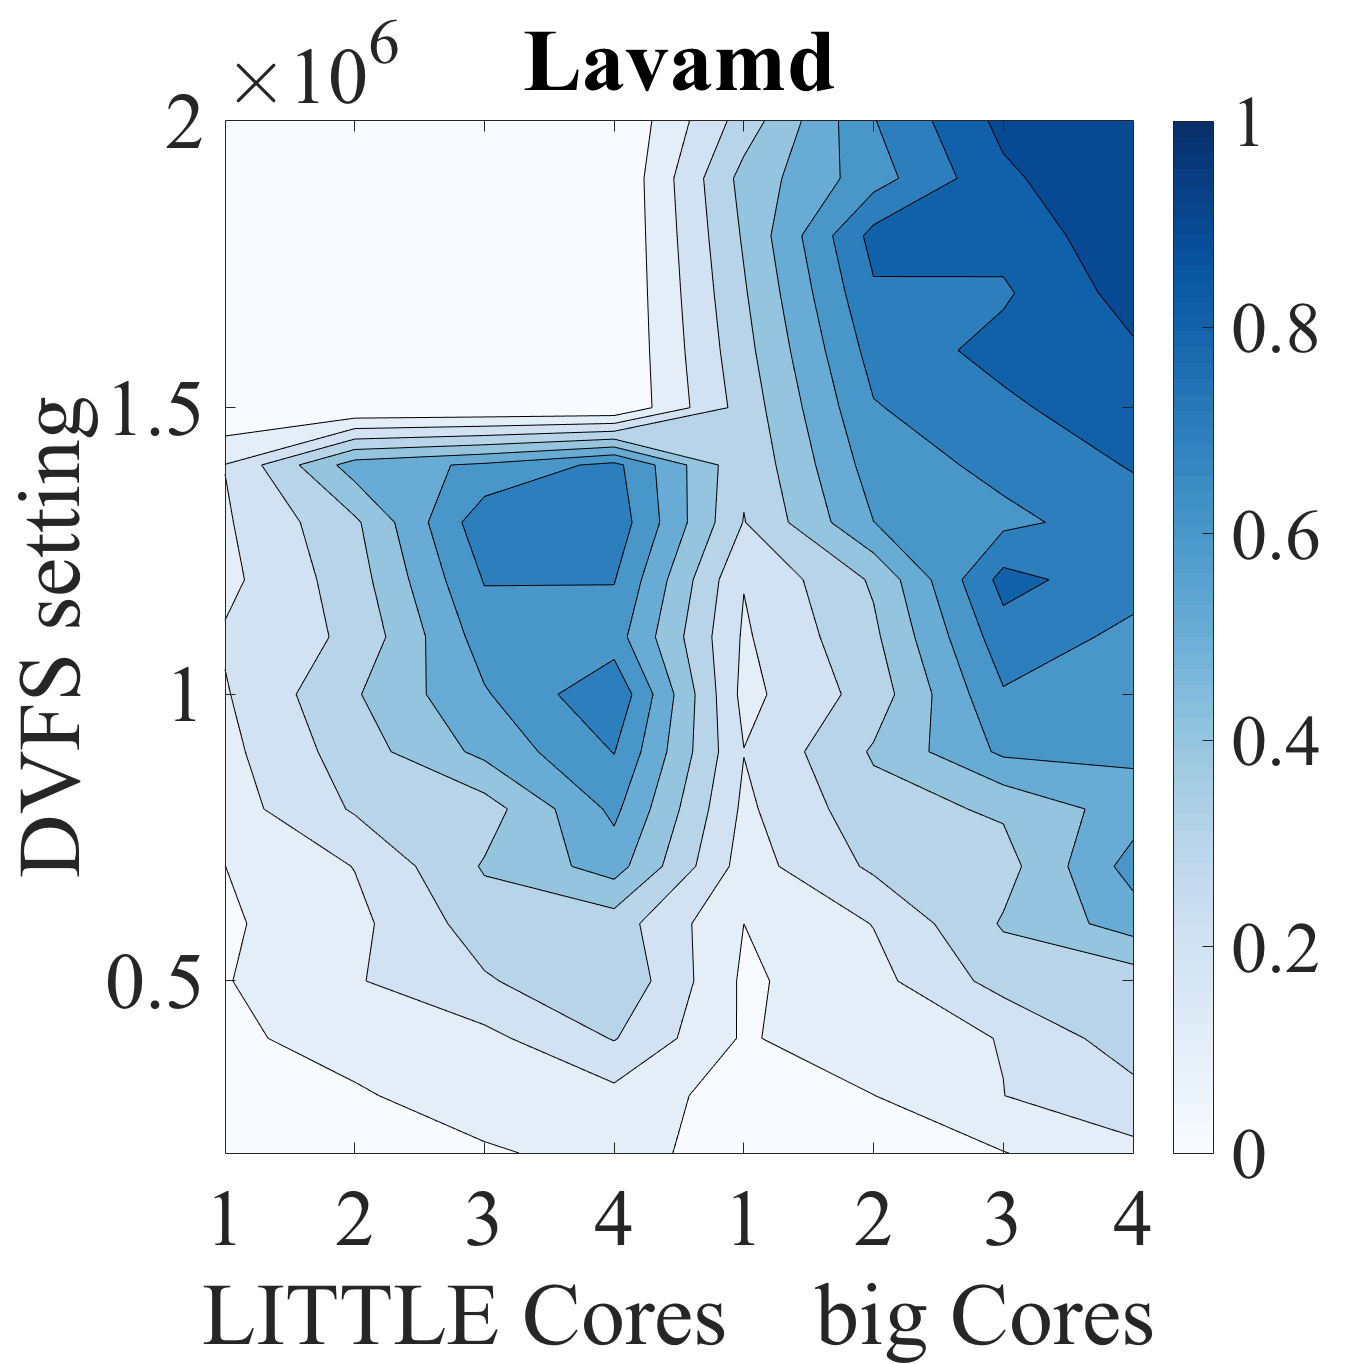
\includegraphics[width=.25\textwidth]{figures/lavamd.png}
%\caption{Performance of LAVAMD with differnt resources.}
%\label{fig:lavamd}
%\end{wrapfigure}
LAVAMD has one of the most complicated responses to resource usage on
our system with multiple local optima, as shown in
\figref{fig:lavamd}.  \secref{guarantees} presents an analytical
argument that tuning the controller to learned variance prevents
oscillation and provide probabilistic control theoretic guarantees
despite using noisy, learned data to control such complicated
behavior.  We now demonstrate this empirically by showing LAVAMD's
single-app behavior controlled by both CALOREE-NoPole and
\SYSTEM{}-HBM to meet the 80\% target.

\figref{fig:lavamd-pole} shows the results, with time on the x-axis
and normalized performance and power on the respective y-axes.
CALOREE-NoPole oscillates around the desired performance and causes
wide fluctuations in power consumption.  In contrast, after receiving
the predictions from its learner, \SYSTEM{} provides reliable
performance right at the target value (normalized to 1 in this case).
\SYSTEM{} also saves tremendous energy because it does not oscillate
but uses a mixture of big and LITTLE cores to keep energy near
minimal.
% \TODO{Do we need the vertical line here?  This is a single app run
%   right?}

%\begin{figure}[t]
%  \begin{tikzpicture}
\begin{centering}

\definecolor{s1}{RGB}{228, 26, 28}
\definecolor{s2}{RGB}{55, 126, 184}
\definecolor{s3}{RGB}{77, 175, 74}
\definecolor{s4}{RGB}{152, 78, 163}
\definecolor{s5}{RGB}{255, 127, 0}

\begin{groupplot}[
    group style={
        group name=plots,
        group size=1 by 2,
        xlabels at=edge bottom,
        xticklabels at=edge bottom,
        vertical sep=5pt
    },
height=3.5cm,
width=0.95\columnwidth,
xmajorgrids,
ymajorgrids,
grid style={dashed},
xmin=0,
xmax=500,
yticklabel pos=left,
enlargelimits=false,
tick align = outside,
tick style={white},
xticklabel shift={-5pt},
yticklabel shift={-5pt},
ylabel shift={-2pt},
ylabel style={align=center},
unbounded coords=jump,
]

\nextgroupplot[ylabel={\footnotesize Performance \\ (Normalized)}, % Performance
%xtick={0,500,1000,1500,2000,2500,3000,3500,4000,4500},
ytick={0.0,0.5,1.0,1.5,2.0},
yticklabels={,0.5,1.0,1.5,2.0},
%xtick={0,30,60,120,160,200,240,280,320,480},
%xticklabels={,0,30,60,120,160,200,240,280,320,480},
yticklabel style={font=\footnotesize},
ymin=0,
ymax=2.0,
legend entries={{$\mathsf{\SYSTEM{}-NP}$},{{$\mathsf{\SYSTEM{}}$}}},
legend style={draw=none,at={(0.5,1.4)},anchor=north,legend columns=4,line width=5pt},
]

\addplot[thick, solid, color=s5] table[x index=0,y index=1,col sep=space] {img/pole/leo-poet-np-LAVAMD.txt};
\addplot[thick, solid, color=s3] table[x index=0,y index=1,col sep=space] {img/pole/leo-poet-LAVAMD.txt};
%\addplot[thick, solid, color=s3] table[x index=0,y index=1,col sep=space] {img/x264-native-ducks/leopoet.txt};

%\addplot[thick, solid, color=s3] table[x index=0,y index=1,col sep=tab] {img/x264-phases-clover-dvfs.txt};
%\addplot[thick, solid, color=s4] table[x index=0,y index=1,col sep=tab] {img/x264-phases-clover-copper.txt};
%\addplot[thick, solid, black] coordinates {(0, 1) (4500, 1)};
\addplot[thick, dashed, black] coordinates {(250,0) (250, 2)};
%\addplot[thick, dashed, black] coordinates {(3000,0) (3000, 2)};


\nextgroupplot[ylabel={\footnotesize Power \\ (Watts)}, % Power
ytick={0.0,2.0,4.0,6.0},
yticklabels={,2.0,4.0,6.0},
yticklabel style={font=\footnotesize},
ymin=0,
ymax=6.0,
xlabel={\footnotesize $time$ [frame]},
xlabel near ticks,
%xtick={0,500,1000,1500,2000,2500,3000,3500,4000,4500},
%xtick={0,30,60,120,160,200,240,280,320,480},
xticklabels={,0,100,200,300,400,500},
%xticklabel style={font=\footnotesize},
]

\addplot[thick, solid, color=s5] table[x index=0,y index=2,col sep=space] {img/pole/leo-poet-np-LAVAMD.txt};
\addplot[thick, solid, color=s3] table[x index=0,y index=2,col sep=space] {img/pole/leo-poet-LAVAMD.txt};
%\addplot[thick, solid, color=s3] table[x index=0,y index=2,col sep=space] {img/x264-native-ducks/leopoet.txt};
%\addplot[thick, solid, color=s3] table[x index=0,y index=2,col sep=tab] {img/x264-phases-clover-dvfs.txt};
%\addplot[thick, solid, color=s4] table[x index=0,y index=2,col sep=tab] {img/x264-phases-clover-copper.txt};
%\addplot[thick, dashed, black] coordinates {(1500,0) (1500, 250)};
%\addplot[thick, dashed, black] coordinates {(3000,0) (3000, 250)};
\addplot[thick, dashed, black] coordinates {(250,0) (250, 6)};
\end{groupplot}
\end{centering}

\end{tikzpicture}

%   \vskip -.5em
%   \caption{The pole's effects on LAVAMD behavior.}
%  \label{fig:lavamd-pole}
%\end{figure}


\subsection{Sensitivity to the Measured Samples}
We vary the number of samples taken and show how it affects learning
accuracy for the Online, Netflix, and HBM learners.  Accuracy is how
close the learner is to ground truth (found through exhaustive
exploration), with 1 meaning the learner perfectly predicted the real
performance or power.  Accuracy is significant because the smaller
the number of samples, the faster the controller can switch to the
learner's application-specific predictions.

\figref{fig:sensitivity} compares the Online, HBM, and Netflix
learners for both performance (top) and power (bottom).  The figure
shows sample size on the x-axis and accuracy on the y-axis.  The HBM
initially performs as well as Offline and as sample size increases,
the accuracy uniformly improves, exceeding 90\% after 20 samples. The
Online approach needs at least 7 samples before it can even generate a
prediction.  As Online receives more samples, its accuracy improves
but never exceeds HBM's for the same number of samples. Netflix is
very noisy for sample sizes, but once the number of samples reaches
about 50, it is competitive with HBM.  These results not only
demonstrate the sensitivity to sample size, they show why
\SYSTEM{}-HBM achieves better results than the other learners.

\begin{figure}[t]
  \begin{tikzpicture}
\begin{centering}
\pgfplotstableread[col sep=space]{img/sample_accuracy-v3.txt}{\datatable}
\begin{groupplot}[
    group style={
        group name=plots,
        group size=1 by 2,
        xlabels at=edge bottom,
        xticklabels at=edge bottom,
        vertical sep=5pt
    },
height=3cm,
width=0.95\columnwidth,
xmajorgrids,
ymajorgrids,
grid style={dashed},
xmin=0,
xmax=100,
yticklabel pos=left,
enlargelimits=false,
tick align = outside,
tick style={white},
xticklabel shift={-5pt},
yticklabel shift={-5pt},
ylabel shift={-2pt},
ylabel style={align=center},
unbounded coords=jump,
]

\nextgroupplot[ylabel={\footnotesize Accuracy\\(Performance)}, % Performance
xtick={0,20,40,60,80,100},
ytick={0.0,0.3,0.6,0.9},
yticklabels={,0.3,0.6,0.9},
yticklabel style={font=\footnotesize},
ymin=0,
ymax=1,
legend entries={{\footnotesize $\mathsf{ONLINE}$},{\footnotesize $\mathsf{HBM}$},{\footnotesize $\mathsf{NETFLIX}$}},
legend style={draw=none,at={(0.5,1.45)},anchor=north,legend columns=4,line width=5pt},
]
\addplot[thick, solid, color=ONLINE-ADAPT] table[x index=0,y index=3] {\datatable};
\addplot[thick, solid, color=HBM-ADAPT]    table[x index=0,y index=1] {\datatable};
\addplot[thick, solid, color=NUCLEAR-ADAPT]  table[x index=0,y index=7] {\datatable};

\nextgroupplot[ylabel={\footnotesize Accuracy\\ (Power)}, % Power
ytick={0.0,0.3,0.6,0.9,1.0},
yticklabels={,0.3,0.6,0.9,},
yticklabel style={font=\footnotesize},
ymin=0,
ymax=1,
xlabel={\footnotesize  \% of samples for training (Out of 128 resource configs).},
xlabel near ticks,
xtick={0,20,40,60,80,100},
xticklabels={0,20,40,60,80,100},
xticklabel style={font=\footnotesize},
]

\addplot[thick, solid, color=ONLINE-ADAPT]    table[x index=0,y index=4] {\datatable};
\addplot[thick, solid, color=HBM-ADAPT]   table[x index=0,y index=2] {\datatable};
\addplot[thick, solid, color=NUCLEAR-ADAPT] table[x index=0,y index=8] {\datatable};

\end{groupplot}
\end{centering}

\end{tikzpicture}

   \vskip -.5em
  \caption{Estimation accuracy versus sample size.}
  \label{fig:sensitivity}
\end{figure}

%\PUNT{

\subsection{Overhead}
\SYSTEM{}'s main source of overhead is sampling where the applications
need to run through a few configurations before \SYSTEM{} can reliably
estimate the entire power and performance frontier. We argue that the
sampling cost can be distributed across devices by asking each of them
to contribute samples for estimation. Once the sampling phase is over,
the HBM is quite fast and can generate an estimate as fast as 500 ms
which is significantly smaller than the time required to run any of
our applications.  Additionally, \SYSTEM{}'s asynchronous
communication means that the controller never waits for the learner.
Using the four ODROIDs in our experimental system, each board only
needs to contribute 4 samples to achieve 90\% accuracy.  In the worst
case (\texttt{facesim}), this sampling overhead is less than 2\%.  For
all other benchmarks it is lower, and for most it is negligible.

The controller requires only a few floating point operations to
execute, plus the table lookups in the PHT.  To evaluate its overhead,
we time 1000 iterations.  We find that it is under 2 microseconds,
which is significantly faster than we can change any resource
allocation on our system.  We conclude that the controller has
negligible impact on performance and energy consumption of the
controlled device.










